\subsection{drittes}

\begin{comment}
  zula Barbara Seite 46
\end{comment}


\[
  P_c=t^2\partial_t+1
\]
$
P_c=t^2\partial_t+1
\Rightarrow
\begin{cases}
  k=1, l=2 & \Rightarrow u \leq 1, v \geq 1\\
  k=0, l=1 & \Rightarrow u \leq 0  v \geq 0\\
\end{cases}
$
\begin{center}
  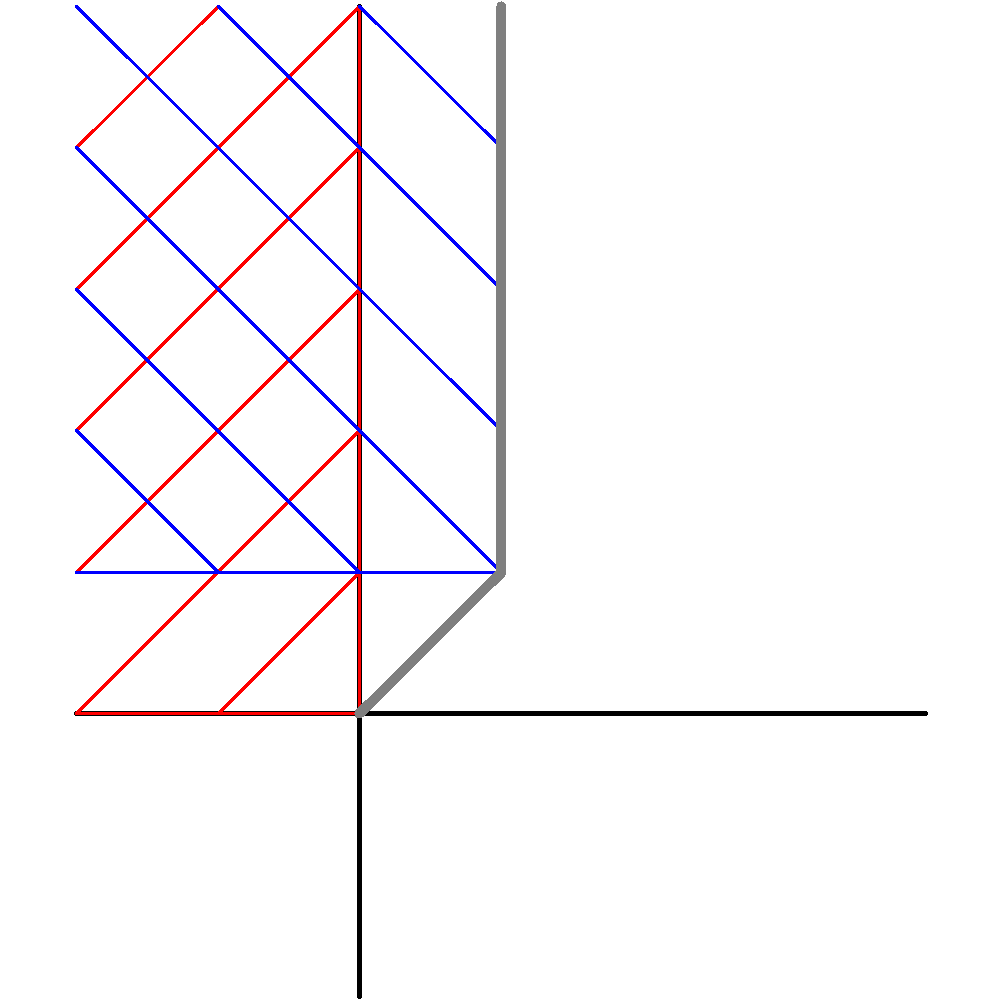
\includegraphics[width=6cm]{img/c.png}
\end{center}

also $\slopes(P_c)=\{1\}$.

% vim:set ft=tex :
